\raggedbottom
\chapter{TINJAUAN PUSTAKA}

Bab ini menguraikan tinjauan pustaka yang mencakup literatur penelitian terdahulu serta landasan teori pokok yang relevan dengan topik pada tugas akhir ini. Pada bagian pertama, dipaparkan ulasan analitis mengenai berbagai studi terkait asesmen kepribadian otomatis sebagai acuan perbandingan untuk menonjolkan kebaruan pendekatan hibrida yang diusulkan. Bagian kedua membahas konsep-konsep fundamental yang mendukung perancangan sistem, mulai dari model psikologi \textit{Big Five personality}, arsitektur \textit{deep learning} berbasis Transformer, teknologi LLM, hingga metrik evaluasi yang digunakan.
% Ubah konten-konten berikut sesuai dengan isi dari tinjauan pustaka
\section{Hasil Penelitian Terdahulu}

Pada subbab ini, akan dibahas mengenai hasil penelitian-penelitian terdahulu yang relevan dengan topik penelitian ini. Hasil berbagai penelitian tersebut digunakan sebagai sumber informasi dan acuan pengembangan metode. Ulasan mengenai perbandingan metode, fokus penelitian, dan modalitas yang digunakan oleh studi-studi tersebut dirangkum secara ringkas dalam \autoref{tab:penelitian-terkait}.

% Tabel Penelitian Terdahulu
{ % Buka grup pengaturan lokal
	\footnotesize
	\renewcommand{\arraystretch}{1.3} % Spasi vertikal (Padding)
	\noindent % Mencegah tabel tergeser ke kanan

	%	\setlength{\LTpost}{0pt}

	% Definisi kolom (Total = 4)
	\begin{xltabular}{\textwidth}{|
			>{\hsize=0.8\hsize}X |
			>{\hsize=1.5\hsize}X |
			>{\hsize=0.7\hsize}X |
			>{\hsize=1.0\hsize}X | }

		% --- CAPTION ---
		\caption{Penelitian Terdahulu} \label{tab:penelitian-terkait} \\
		\hline

		% --- HEADER HALAMAN PERTAMA ---
		\multicolumn{1}{|>{\centering\arraybackslash\hsize=0.8\hsize}X|}{\bfseries Judul} &
		\multicolumn{1}{>{\centering\arraybackslash\hsize=1.5\hsize}X|}{\bfseries Fokus Utama Penelitian} &
		\multicolumn{1}{>{\centering\arraybackslash\hsize=0.7\hsize}X|}{\bfseries Modalitas} &
		\multicolumn{1}{>{\centering\arraybackslash\hsize=1.0\hsize}X|}{\bfseries Perbedaan dengan Tugas Akhir yang Diusulkan} \\ \hline
		\endfirsthead

		% --- HEADER HALAMAN LANJUTAN ---
		\caption*{Lanjutan Tabel \ref{tab:penelitian-terkait}} \\
		\hline
		\multicolumn{1}{|>{\centering\arraybackslash\hsize=0.8\hsize}X|}{\bfseries Judul} &
		\multicolumn{1}{>{\centering\arraybackslash\hsize=1.5\hsize}X|}{\bfseries Fokus Utama Penelitian} &
		\multicolumn{1}{>{\centering\arraybackslash\hsize=0.7\hsize}X|}{\bfseries Modalitas} &
		\multicolumn{1}{>{\centering\arraybackslash\hsize=1.0\hsize}X|}{\bfseries Perbedaan dengan Tugas Akhir yang Diusulkan} \\ \hline
		\endhead
		
		\hline
		\multicolumn{4}{r}{\textit{Berlanjut ke halaman berikutnya...}} \\
		\endfoot

		% --- FOOTER ---
		\hline
		\endlastfoot

		% --- ISI DATA ---
		\textit{A multi-modal personality prediction system} \parencite{Suman2022} &
		Mengembangkan sistem prediksi kepribadian multimodal menggunakan arsitektur CNN tradisional (ResNet, MTCNN, VGGish CNN) dan teknik \textit{early fusion}. Fusi fitur \textit{concantenation} yang diekstrak dari berbagai modalitas menghasilkan kinerja yang sebanding dengan metode rata-rata prediksi \textit{late fusion}. &
		Gambar, audio, dan teks anotasi dari dataset ChaLearn \parencite{Ponce-Lpez2016}. &
		Tugas akhir ini menggunakan arsitektur Transformer untuk prediksi kepribadian dengan modalitas gambar dan fokus utama pada interpretasi deskriptif berbasis LLM. \\ \hline

		\textit{A Systematic Approach for the Prediction of Personality Based on Attention Enhanced GCNN and LSTM Approach} \parencite{Sharma2023} &
		Mengembangkan sistem prediksi kepribadian berbasis teks menggunakan AGCNN-LSTM untuk mengatasi kekurangan dari algoritma \textit{deep learning} yang ada seperti CNN dan LSTM dalam hal kecepatan pelatihan dan kemampuan menangkap makna semantik. &
		Konten tekstual dari unggahan media sosial (tf-idf). &
		Tugas akhir ini menggunakan arsitektur Transformer dengan modalitas gambar yang bisa menangkap konteks global yang lebih luas menggunakan mekanisme \textit{self-attention}. \\ \hline

		\textit{An Effective Personality Prediction using Bidirectional Encoder Representations from Transformers with AdamW Optimizer} \parencite{Devi2024} &
		Mengembangkan model prediksi kepribadian MBTI berbasis teks menggunakan BERT dan AdamW \textit{Optimizer} untuk ekstraksi fitur, dengan \textit{Linear Regression} untuk prediksi akhir. &
		Teks, berasal dari dataset MBTI yang berisi esai yang telah dianotasi. &
		Tugas akhir ini berfokus pada prediksi kepribadian \textit{Big Five} berbasis visual/gambar dan menggunakan LLM untuk interpretasi kualitatif hasil prediksi. \\ \hline
		
		\textit{PersonaLLM: Investigating the Ability of Large Language Models to Express Personality Traits} \parencite{Jiang2024} &
		Menginvestigasi kemampuan LLM (GPT-3.5 dan GPT-4) untuk secara akurat dan konsisten merefleksikan profil kepribadian \textit{Big Five} yang ditetapkan melalui tes BFI dan penulisan cerita. &
		Narasi teks yang dihasilkan oleh LLM. &
		Tugas akhir ini menggunakan LLM sebagai alat interpretasi generatif yang menerima hasil prediksi visual sebagai input. \\ \hline

		\textit{Prediction of Personality Traits and Suitable Job through an Intelligent Interview Agent using Machine Learning} \parencite{Mandakini2023} &
		Memprediksi skor \textit{big five personality} dari video wawancara menggunakan model CNN (VGG16), kemudian mengklasifikasikan peran pekerjaan yang sesuai. &
		Video dari wawancara. &
		Tugas akhir ini berfokus pada interpretasi psikologis kualitatif dari prediksi kepribadian \textit{Big Five} menggunakan arsitektur Transformer dan LLM. \\ \hline
		
		Prediksi Kepribadian Berbasis Gambar Wajah Dengan Arsitektur \textit{Dual-Branch Adaptive Distribution Fusion} Dan Integrasi Fitur Emosi \parencite{Aryan2025} & Mengusulkan arsitektur \textit{dual-branch Adaptive Distribution Fusion} (Ada-DF) untuk memprediksi lima dimensi kepribadian \textit{Big Five}. Fitur emosi diintegrasikan pada Ada-DF untuk memperkaya representasi data. & Gambar wajah yang diambil dari dataset Chalearn \parencite{Ponce-Lpez2016}. & Tugas akhir ini menggunakan model berbasis Transformer dengan arsitektur \textit{custom regression head} untuk memprediksi kepribadian \textit{Big Five}. Wajah pada \textit{frame} diekstraksi menggunakan BlazeFace \\ \hline
		
		Prediksi Kepribadian Berbasis Fitur Visual Menggunakan Arsitektur Swin Transformer Dan \textit{Multi-Frame Aggregation} \parencite{Wildan2026} & Mengembangkan model prediksi kepribadian berbasis fitur visual wajah menggunakan arsitektur Swin Transformer dan strategi \textit{Multi-Frame Aggregation}. Penelitian juga mengintegrasikan fitur emosi, \textit{frame attention}, \textit{temporal transformer}, \textit{quality-weighted loss}, serta \textit{face embedding} berbasis ArcFace guna meningkatkan kualitas representasi wajah. & Gambar yang diekstraksi dari video pada dataset Chalearn \parencite{Ponce-Lpez2016} & Tugas akhir ini menggunakan 15 \textit{frame} yang diekstrak dari video dan setiap \textit{frame} dianggap sebagai data independen dengan label yang sama. Selanjutnya dilakukan prediksi dan interpretasi menggunakan Transformer dan LLM. \\ \hline
		
		Evaluasi Fitur \textit{Handcrafted} dan Model \textit{Speech} Pralatih untuk Estimasi Kepribadian Big Five Berbasis Audio pada Protokol \textit{Strict Split} serta Analisis \textit{Fine-Tuning} Berbasis LoRA \parencite{Aqil2026} & Memprediksi nilai kepribadian \textit{Big Five} membandingkan fitur \textit{handcrafted} eGeMAPS dengan \textit{embedding model speech} pralatih wav2vec 2.0, HuBERT, dan WavLM dalam skema \textit{frozen feature extraction} menggunakan \textit{Ridge Regression}. Selain itu, dilakukan \textit{fine-tune} berbasis LoRA pada WavLM dan HuBERT. & Audio dari dataset ChaLearn \parencite{Ponce-Lpez2016} & Tugas akhir ini menggunakan modalitas visual video dari dataset yang dilakukan praproses menjadi gambar untuk memprediksi nilai kepribadian \textit{Big Five} menggunakan model berbasis Transformer. \\ \hline
		
		Prediksi \textit{Big Five Personality} pada Video Monolog Singkat Berbasis Video Transformer \parencite{Adyuta2026} & Memprediksi lima nilai \textit{Big Five Personality} menggunakan ViViT, TimeSformer, dan VideoMAE yang telah dilatih pada dataset Kinetics-400. &  Visual berupa urutan \textit{frame} wajah dari dataset ChaLearn \parencite{Ponce-Lpez2016}. & Tugas akhir ini menggunakan modalitas gambar statis yang diekstraksi dari video untuk memprediksi nilai kepribadian \textit{Big Five}. \\ \hline	

	\end{xltabular}
} % Tutup grup pengaturan lokal

%\vspace{-1em}

Penelitian \textcite{Suman2022} bertujuan untuk mengembangkan sistem prediksi kepribadian otomatis/\textit{Automatic Personality Prediction} (APP) dengan memanfaatkan berbagai modalitas data, termasuk visual, audio, dan teks (transkrip) dari video. Ekstraksi fitur dilakukan menggunakan arsitektur CNN yang sudah ada seperti ResNet dan MTCNN untuk modalitas visual, VGGish CNN untuk audio, dan CNN berbasis n-gram untuk fitur teks. Fitur-fitur ini kemudian digabungkan menggunakan strategi \textit{early fusion} (konkatensi fitur) atau \textit{late fusion} (rata-rata prediksi). Fokus penelitian adalah mencapai akurasi prediksi yang tinggi sebagai tugas regresi. Kelemahan utamanya adalah ketergantungan pada arsitektur CNN tradisional untuk pemrosesan fitur visual. Namun, pendekatan ini masih bergantung pada CNN tradisional yang belum memanfaatkan mekanisme \textit{self-attention} seperti Transformer yang dapat meningkatkan representasi fitur visual \parencite{El-Demerdash2022}. Selain itu, penelitian ini tidak menyentuh aspek interpretasi naratif dari skor prediksi yang dihasilkan.

Penelitian oleh \textcite{Sharma2023} berfokus pada prediksi kepribadian menggunakan konten tekstual dari media sosial dengan model hibrida AGCNN-LSTM (\textit{Attention Enhanced Graph Convolution Neural Network dan Long Short-Term Memory}) yang dirancang untuk mengatasi keterbatasan CNN dan LSTM konvensional, seperti waktu pelatihan yang lama dan kesulitan dalam menangkap makna semantik kata. Model ini menunjukkan performa yang unggul dibandingkan model-model yang menjadi \textit{baseline}. Meskipun menyajikan solusi hibrida yang kuat, model ini masih didasarkan pada arsitektur sekuensial LSTM yang kurang efisien dalam pemrosesan konteks global dan paralel dibandingkan Transformer \parencite{Prasad2024}. Selain itu, fokus penelitian ini hanya pada modalitas teks, sementara beberapa studi lain menunjukkan bahwa dengan menggunakan serta menggabungkan modalitas lain seperti gambar/visual, dapat meningkatkan akurasi prediksi kepribadian.

Studi oleh \textcite{Jiang2024} menyelidiki kemampuan LLM seperti GPT-3.5 dan GPT-4 untuk merefleksikan dan meniru ciri-ciri kepribadian \textit{Big Five}. Penelitian ini menggunakan LLM sebagai persona untuk menyelesaikan tes kepribadian dan menghasilkan narasi pribadi yang kemudian dianalisis menggunakan fitur psikolinguistik LIWC. Hasil penelitian menunjukkan LLM dapat menampilkan kepribadian yang konsisten. Penelitian ini memiliki keterbatasan karena sebagian besar analisisnya terfokus pada model tertutup dan modalitas teks, sehingga konteks multimodal atau interaksi yang lebih dinamis belum tereksplorasi \parencite{Tseng2024}. Studi ini juga mencatat bahwa kesadaran manusia terhadap penulis AI dapat memengaruhi persepsi terhadap kepribadian yang ditampilkan sehingga menimbulkan tantangan dalam evaluasi yang objektif.

Penelitian \textcite{Devi2024} mengusulkan model berbasis \textit{Bidirectional Encoder Representations from Transformers} (BERT) dengan AdamW \textit{Optimizer} untuk ektraksi fitur prediksi kepribadian berbasis teks. Data yang digunakan adalah dataset MBTI. Praproses data seperti \textit{lemmatiozation} dan \textit{lowercasing} dilakukan terlebih dahulu, kemudian data diproses dengan model BERT untuk ekstraksi fitur atribut yang optimal, dilanjutkan dengan prediksi menggunakan \textit{Linear Regression}. Model ini menunjukkan akurasi yang lebih unggul dibandingkan dengan model sekuensial seperti LSTM. Meskipun menggunakan Transformer pada prosesnya, model ini hanya digunakan untuk melakukan ekstraksi fitur modalitas tekstual yang menghasilkan atribut optimal untuk dilakukan prediksi menggunakan model tradisional.

Penelitian \textcite{Mandakini2023} berfokus pada pengembangan agen wawancara cerdas yang menggunakan \textit{machine learning} untuk memprediksi kepribadian \textit{Big Five} dari video wawancara. Model ini menggunakan input citra wajah yang diambil dari \textit{frame} pada video wawancara dan mengaplikasikan model CNN VGG-16 untuk prediksi kepribadian \textit{Big Five}. Tujuan dari penelitian ini adalah untuk memprediksi kecocokan pekerjaan berdasarkan hasil prediksi kepribadian. Kekurangan penelitian ini adalah prediksi hanya berfokus pada nilai numerik serta klasifikasi pekerjaan numerik yang sesuai. Selain itu, inferensi deskriptif yang ditunjukkan dari model hanya berupa kategorisasi berdasarkan nilai luaran dari model, misal nilai (0-0,4) pada sifat \textit{openness} dikategorikan sebagai \textit{low} sedangkan nilai (0,5-1,0) dikategorikan sebagai \textit{high} sehingga tidak menunjukkan interpretasi antar sifat \textit{Big Five} yang kualitatif secara mendalam.


\section{Dasar Teori}

Subbab ini memaparkan berbagai konsep fundamental dan teori keilmuan yang menjadi landasan utama dalam penyusunan tugas akhir ini. Pembahasan mencakup teori psikologi mengenai \textit{Big Five personality} serta tinjauan mendalam mengenai arsitektur \textit{deep learning} yang digunakan, meliputi Transformer dan LLM. Selain itu, subbab ini juga menjelaskan tentang teknik pemrosesan data wajah, detail mengenai dataset ChaLearn, hingga metrik evaluasi yang digunakan untuk mengukur kinerja sistem.

\subsection{\textit{Big Five Personality}}

Kepribadian didefinisikan sebagai kumpulan perbedaan individu yang biasa disebut ciri psikologis dalam diri individu yang menjelaskan pola proses dan mental yang menentukan penyesuaian unik terhadap lingkungan, mencakup pola pikir, perasaan, dan perilaku yang relatif stabil sepanjang waktu \parencite{Phan2021}. Pada psikologi kepribadian, model \textit{Big Five} muncul sebagai paradigma paling dominan karena sifatnya yang konsisten dan universal \parencite{Ponce-Lpez2016}. Model ini mendefinisikan kepribadian manusia ke dalam lima dimensi yang sering disingkat OCEAN, yaitu \textit{Openness, Conscientiousness, Extraversion, Agreeableness,} dan \textit{Neuroticism}. Dimensi \textit{Openness} mencerminkan tingkat imajinasi, keingintahuan intelektual, serta kesediaan untuk menerima ide dan pengalaman baru. \textit{Conscientiousness} menggambarkan sejauh mana seseorang dapat bertanggung jawab, menjaga disiplin diri, dan berorientasi pada pencapaian tujuan yang sering kali menjadi aspek penting bagi kinerja akademik maupun pekerjaan. \textit{Extraversion} menunjukkan kuantitas dan intensitas interaksi sosial yang ditandai dengan sifat ramah, tegas, serta kecenderungan untuk mencari stimulasi sosial. \textit{Agreeableness} menilai kualitas orientasi interpersonal, mulai dari sikap lembut, kooperatif, dan penuh kepercayaan hingga kecenderungan antagonistik. Dimensi terakhir, yaitu \textit{Neuroticism} merefleksikan ketidakstabilan emosi dan kerentanan terhadap emosi negatif seperti kecemasan dan depresi \parencite{Zell2022}.

\subsection{\textit{ChaLearn First Impressions}}

\textit{ChaLearn First Impression} merupakan dataset yang digunakan untuk melakukan evaluasi otomatis terhadap ciri kepribadian tampak (\textit{apparent personality trait}) berdasarkan penilaian manusia \parencite{Ponce-Lpez2016}. Dataset ini dikembangkan untuk kompetisi \textit{ChaLearn Looking at People} yang bertujuan untuk mengatasi kurangnya data yang konsisten dalam prediksi kepribadian. Dataset ini terdiri dari 10000 klip video pendek dengan durasi rata-rata 15 detik yang diekstrak dari kurang lebih 3000 video HD YouTube mengenai orang-orang dari berbagai keragaman gender, usia, etnis, dan kebangsaan. 

Subjek dalam video berbicara mengenai presentasi diri yang menyerupai wawancara di depan kamera seperti yang ditunjukkan pada Gambar \ref{fig:chalearn-dataset}. Setiap klip video diberi label yang didasarkan pada model kepribadian \textit{Big Five} yang mencakup \textit{Openness, Conscientiousness, Extraversion, Agreeableness,} dan \textit{Neuroticism}, dengan tambahan satu variabel \textit{interview} pekerjaan. Label tersebut diperoleh melalui penilaian persepsi pengamat manusia menggunakan platform \textit{Amazon Mechanical Turk} (AMT). Penilaian tersebut kemudian direpresentasikan dalam rentang 0 hingga 1 untuk setiap karakteristik kepribadian \textit{Big Five}.

\begin{figure}[H]
	\centering
	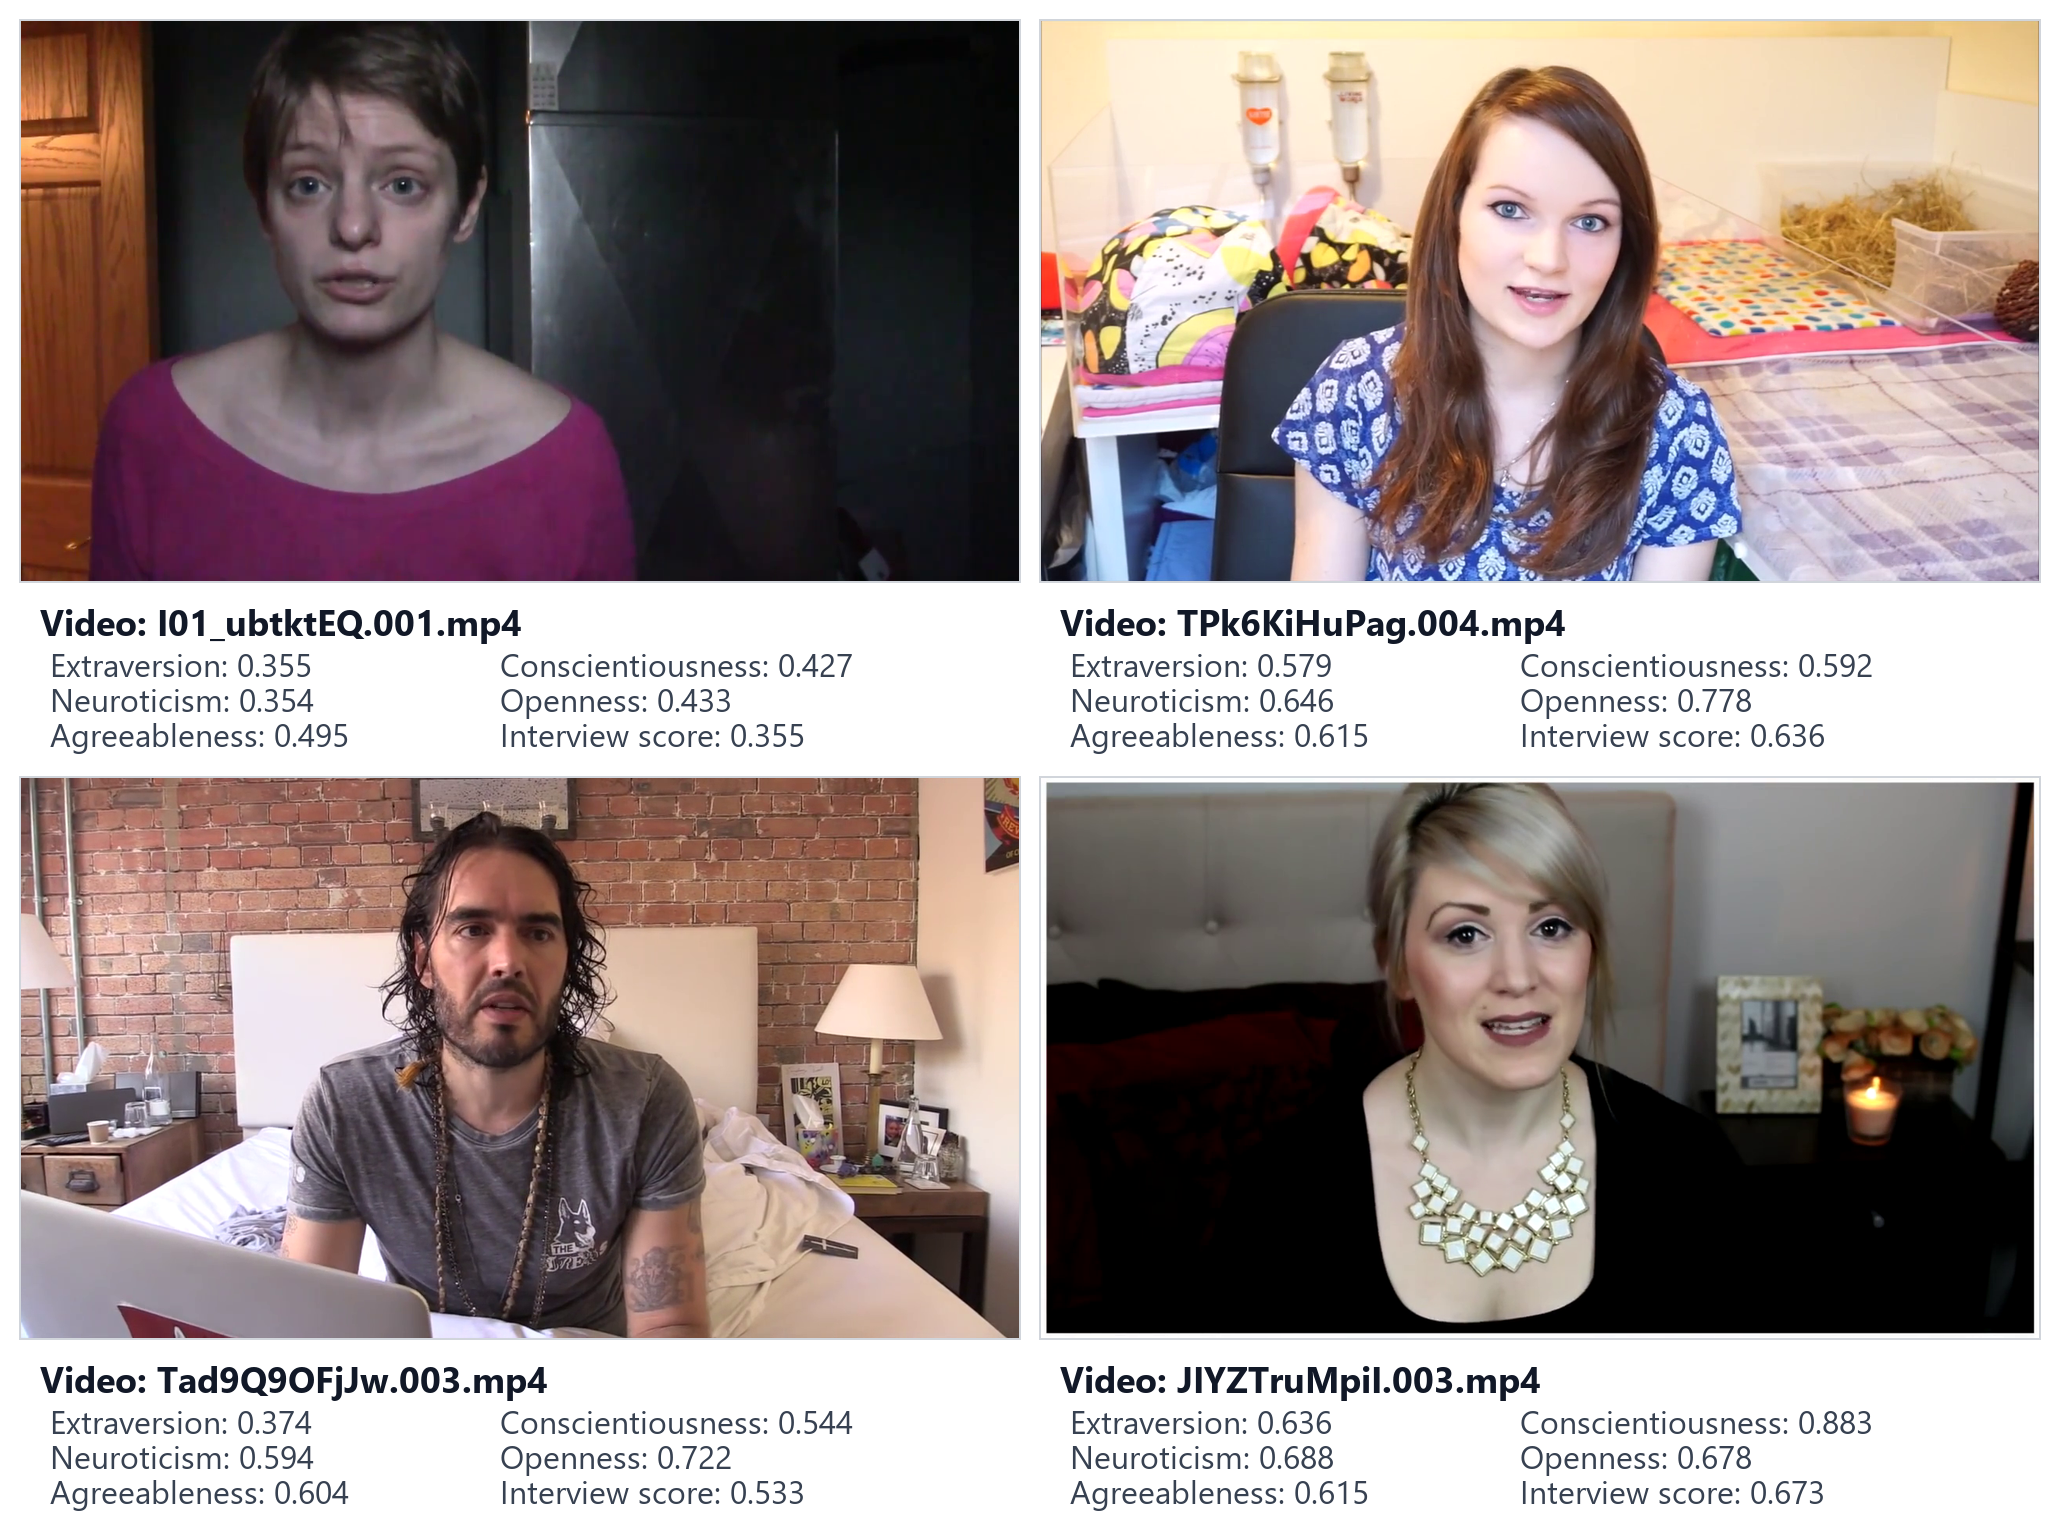
\includegraphics[width=0.8\linewidth]{gambar/chalearn-dataset.png}
	\caption{Cuplikan Video dengan Label pada Dataset ChaLearn}
	\label{fig:chalearn-dataset}
\end{figure}

\subsection{\textit{Deep Learning}}

\textit{Deep Learning} merupakan bagian dari \textit{machine learning} yang menggunakan jaringan saraf berlapis untuk menyimulasikan proses pembelajaran pada otak manusia dalam memodelkan pola data tingkat tinggi \parencite{Taye2023}. Fondasi utama dari teknologi ini adalah neuron buatan (\textit{perceptron}) yang merupakan unit pemrosesan kecil yang menerima berbagai input untuk menghasilkan sebuah \textit{output}. Setiap input yang diterima oleh neuron diberikan bobot (\textit{weight}) tertentu yang mencerminkan tingkat signifikansi input tersebut terhadap keputusan akhir model. Setiap neuron memiliki parameter bias yang berfungsi untuk mengatur \textit{output} agar model dapat mencapai kecocokan data yang paling optimal \parencite{Sarker2021, Taye2023}. Gambar \ref{fig:perceptron} menggambarkan model matematika dari \textit{perceptron}, di mana seluruh input dengan bobot dan bias dijumlahkan melalui \textit{summation function} sebelum diproses lebih lanjut.

\begin{figure}[H]
	\centering
	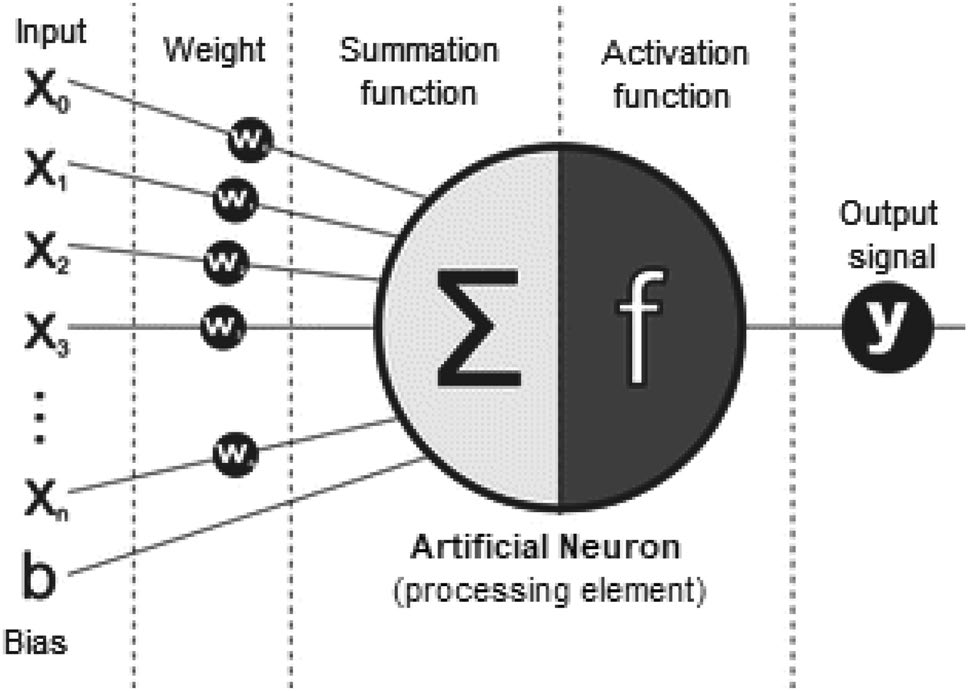
\includegraphics[width=0.5\linewidth]{gambar/perceptron.png}
	\caption{Representasi Model Matematika Neuron Buatan (\textit{Perceptron}) \parencite{Sarker2021}}
	\label{fig:perceptron}
\end{figure}

\textit{Deep neural network} atau dikenal juga dengan \textit{feed-forward neural network} merupakan sebuah jaringan di mana data diproses dari lapisan input kemudian menuju lapisan tersembunyi (\textit{hidden layer}) dan berakhir di lapisan \textit{output}. Fungsi aktivasi seperti ReLU, Sigmoid, Tanh, atau Softmax berperan penting dalam proses ini dengan memberikan sifat \textit{non-linear} sehingga \textit{neural network} mampu mempelajari hubungan data yang sangat kompleks \parencite{Taye2023}. Untuk mengukur kinerja model dalam melakukan prediksi dengan benar, digunakan \textit{loss function} yang bertugas menghitung selisih atau kesalahan antara hasil prediksi model dengan label target yang sebenarnya. Beberapa jenis \textit{loss function} yang umum digunakan meliputi \textit{Cross-Entropy} untuk tugas klasifikasi dan \textit{Mean Square Error} untuk tugas regresi \parencite{Alzubaidi2021}.

Salah satu proses krusial dalam \textit{deep learning} adalah optimasi, yaitu proses memperbarui parameter internal model seperti \textit{weight} dan bias secara iteratif untuk meminimalkan nilai \textit{loss function} \parencite{Abdulkadirov2023, Alzubaidi2021}. Proses ini dijalankan menggunakan algoritma \textit{backpropagation} yang menghitung turunan parsial atau gradien untuk menentukan arah penyesuaian parameter yang paling efisien \parencite{Sarker2021, Taye2023}. Algoritma Adam (\textit{Adaptive Moment Estimation}) merupakan salah satu \textit{optimizer} yang sering digunakan karena efisiensinya dalam menghitung laju pembelajaran adaptif menggunakan rata-rata \textit{exponential moving} dari gradien dan kuadrat gradien \parencite{Abdulkadirov2023, Alzubaidi2021}. Untuk meningkatkan kemampuan generalisasi model, dikembangkan varian AdamW yang secara spesifik mengintegrasikan regularisasi L2 dengan cara memisahkan mekanisme \textit{weight decay} dari langkah \textit{update} gradien utama. Pendekatan ini memastikan bahwa pengurangan bobot dilakukan secara langsung pada parameter tanpa dipengaruhi oleh penskalaan gradien adaptif \parencite{Abdulkadirov2023}.

\subsection{Deteksi dan Ekstraksi Wajah}

Dalam analisis kepribadian berbasis visual, deteksi dan ekstraksi wajah pada gambar maupun video merupakan tahap praproses yang penting untuk meningkatkan kinerja model dalam melakukan prediksi agar fitur visual yang digunakan tetap relevan. Proses ekstraksi wajah dilakukan menggunakan model BlazeFace yang ringan dalam mendeteksi wajah pada gambar. Model deteksi wajah ini dibangun dengan mengadaptasi arsitektur \textit{Single Shot MultiBox Detector} (SSD) yang dapat memprediksi skor deteksi objek serta melakukan penyesuaian pada kotak pembatas/\textit{bounding box} secara cepat dan akurat tanpa memerlukan teknik yang menggunakan \textit{region proposal} maupun \textit{pooling} seperti pada model Faster R-CNN \parencite{Liu2016}. Selain memprediksi \textit{bounding box} wajah, BlazeFace juga menghasilkan 6 titik koordinat kunci wajah yang dapat digunakan untuk menyelaraskan wajah untuk digunakan pada proses prediksi berikutnya \parencite{Bazarevsky2019}. 

Sistem pelacakan wajah atau \textit{face tracking} diperlukan pada tahap praproses video, mengingat terdapat kemungkinan sebuah video dapat memuat lebih dari satu wajah pada satu \textit{frame}. Mekanisme ini digunakan untuk mempertahankan konsistensi hasil pelacakan wajah target pada \textit{frame-frame} yang berurutan dari awal hingga akhir video. Berdasarkan kerangka kerja \textit{Simple Online and Realtime Tracking} (SORT), pelacakan objek multi target yang efisien dan andal dapat dicapai dengan mengasosiasikan informasi geometri dari \textit{bounding box} pada setiap \textit{frame}. Pendekatan ini dapat diaplikasikan pada deteksi wajah dengan menggunakan titik pusat koordinat \textit{bounding box} dan dimensi ukuran wajah dari hasil ekstraksi pada \textit{frame} yang berurutan untuk membentuk asosiasi data tanpa perlu menambahkan fitur wajah tambahan yang tampak (\textit{appearance features}) yang dapat menambah beban komputasi \parencite{Bewley2017}. Pendekatan pelacakan spasial antar \textit{frame} ini menjamin bahwa hasil ekstraksi akan selalu konsisten untuk wajah yang sama dalam satu video.

Penentuan wajah utama yang akan digunakan dalam sistem pelacakan wajah pada \textit{frame} awal perlu dilakukan dengan mempertimbangkan perhatian visual (\textit{visual attention}) pada objek yang menonjol pada gambar \parencite{Liu2011}. Penentuan ini didasarkan pada titik keseimbangan antara dominasi visual dan fenomena bias pusat (\textit{center prior}). Dominasi visual ditunjukkan oleh seberapa besar ukuran area wajah tersebut di dalam gambar beserta seberapa tinggi tingkat kepercayaan (\textit{confidence score}) yang dihasilkan oleh detektor. Sedangkan bias pusat menunjukkan kecenderungan alami manusia untuk membidik dan memosisikan objek yang paling penting di bagian tengah gambar. Penelitian mengenai pelacakan mata menunjukkan bahwa terdapat bias yang sangat kuat pada perhatian visual manusia yang sebagian besar menunjukkan kecenderungan melihat pada area tengah suatu gambar \parencite{Judd2009}. Berdasarkan penelitian ini, wajah dengan ukuran area yang besar dan memiliki jarak titik pusat \textit{bounding box} terdekat dengan titik pusat keseluruhan \textit{frame} gambar dapat dievaluasi sebagai wajah utama untuk selanjutnya terus dilacak pada \textit{frame} video berikutnya.          

\subsection{Transformer}

Transformer merupakan arsitektur \textit{deep learning} yang dikenalkan oleh \textcite{Vaswani2023} untuk menangani tugas-tugas dalam \textit{Natural Language Processing} (NLP). Arsitektur ini menjadi standar baru karena kemampuannya menggantikan model sekuensial seperti \textit{Recurrent Neural Networks} (RNN) melalui mekanisme \textit{self-attention} \parencite{Vaswani2023}. Transformer memungkinkan komputasi paralel yang masif karena tidak memproses data secara langkah demi langkah, melainkan secara simultan untuk seluruh urutan input. Hal ini memberikan keunggulan signifikan dalam menangkap \textit{long-range dependencies} dan meningkatkan efisiensi waktu pelatihan pada dataset dengan skala besar \parencite{Liu2021}.

Struktur inti Transformer terdiri dari \textit{encoder} dan \textit{encoder}. \textit{Encoder} bertugas memetakan representasi simbol dari \textit{input sequence} menjadi \textit{continuous sequence}. Selanjutnya \textit{decoder} menghasilkan simbol \textit{output sequence} satu per satu secara autoregresif dengan menggunakan simbol-simbol yang dihasilkan sebelumnya sebagai \textit{input} tambahan saat menghasilkan simbol berikutnya \parencite{Vaswani2023}.

\begin{figure}[H]
	\centering
	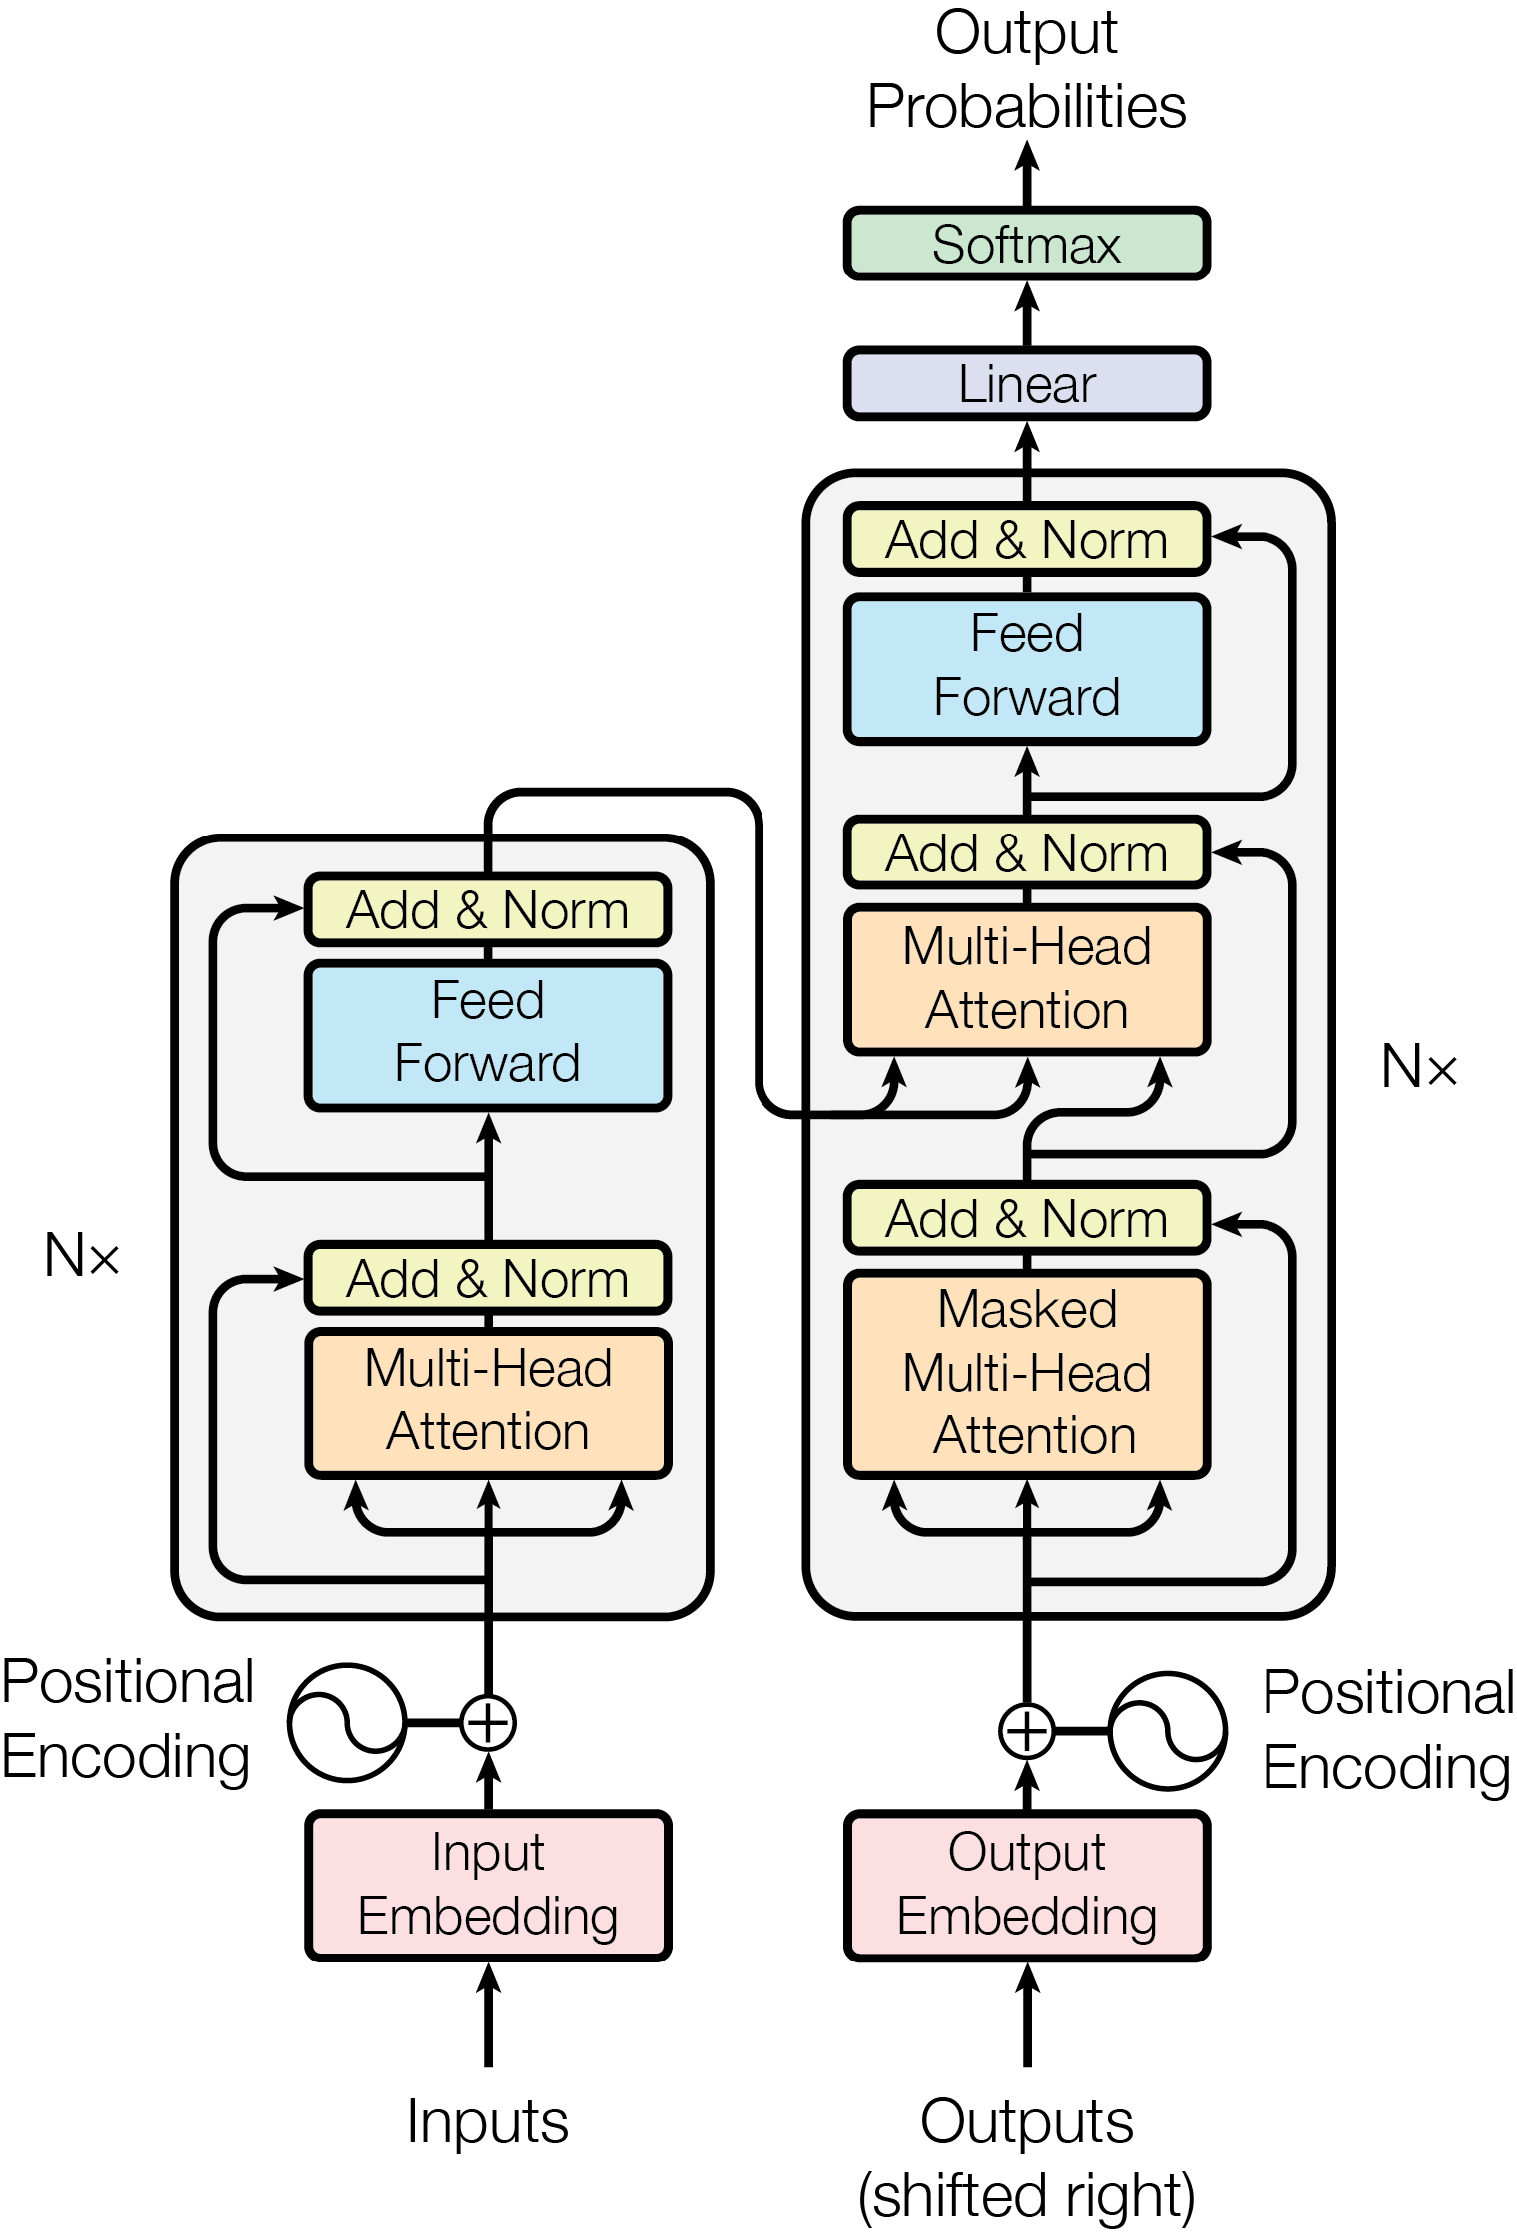
\includegraphics[width=0.45\linewidth]{gambar/transformer.png}
	\caption{Arsitektur Transformer \parencite{Vaswani2023}}
	\label{fig:transformer-arch}
\end{figure}

Secara umum, gambaran arsitektur Transformer ditunjukkan pada Gambar \ref{fig:transformer-arch}. Transformer menggunakan tumpukan \textit{layer self-attention} dan \textit{point-wise fully connected} pada bagian \textit{encoder} maupun \textit{decoder}. \textit{Encoder} terdiri dari \textit{N-layer} yang identik. Setiap \textit{layer} memiliki dua \textit{sub-layer} utama, yaitu \textit{multi-head attention} dan \textit{position-wise fully connected feed-forward network}. Struktur \textit{decoder} juga terdiri dari \textit{N-layer} identik seperti \textit{encoder} dengan tambahan \textit{sub-layer} ketiga yaitu \textit{multi-head attention} di atas hasil \textit{output encoder}. Setiap \textit{sub-layer} menerapkan koneksi residual yang diikuti oleh \textit{layer normalization}. Mekanisme \textit{self-attention} pada \textit{decoder} dimodifikasi dengan \textit{masking} untuk mencegah suatu posisi memperhatikan posisi-posisi setelahnya pada saat proses generasi. Hal ini memastikan bahwa hasil prediksi pada posisi $i$ hanya bergantung pada \textit{output} yang diketahui pada posisi kurang dari $i$ sehingga mempertahankan sifat autoregresif model. Karena model ini tidak menggunakan rekurensi maupun konvolusi, maka digunakan \textit{positional encoding} pada bagian bawah \textit{stack encoder} dan \textit{decoder} untuk memberikan informasi mengenai urutan posisi relatif maupun absolut dari setiap token dalam rangkaian data. Sistem ini memungkinkan setiap posisi pada \textit{decoder} memerhatikan seluruh posisi pada \textit{input sequence} sekaligus mempertahankan efisiensi dengan komputasi paralel \parencite{Vaswani2023}.

\subsection{Vision Transformer (ViT)}

Vision Transformer (ViT) merupakan arsitektur yang mengadaptasi model Transformer untuk digunakan pada ranah \textit{computer vision} dengan mengubah citra gambar menjadi urutan \textit{patch} \parencite{Han2023}. ViT menggunakan mekanisme \textit{self-attention} dan \textit{multi-head self-attention} untuk memodelkan hubungan global antar bagian citra sehingga dapat menangkap dependensi jarak jauh secara eksplisit \parencite{Khan2022, Thisanke2023}. Secara umum, ViT memperlakukan citra dua dimensi sebagai urutan token (\textit{patch} citra) dan memprosesnya dengan \textit{encoder} Transformer standar sehingga struktur dasarnya mirip dengan Transformer untuk NLP yang ditambahkan tahap tokenisasi citra dan penambahan \textit{positional embedding} \parencite{Wang2025}.

\begin{figure}[H]
	\centering
	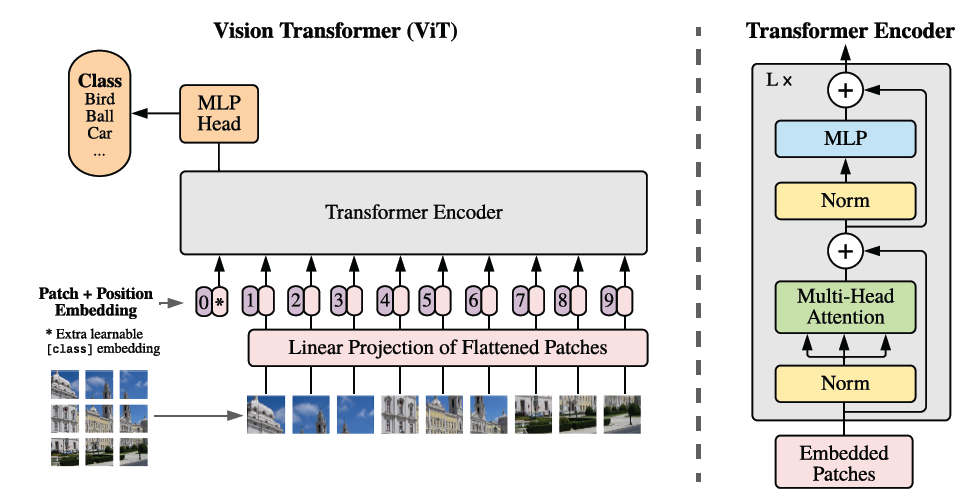
\includegraphics[width=0.9\linewidth]{gambar/ViT.png}
	\caption{Arsitektur Vision Transformer \parencite{Dosovitskiy2021}}
	\label{fig:vit-arch}
\end{figure}

Berdasarkan \autoref{fig:vit-arch}, proses ViT dimulai dengan membagi citra input dua dimensi menjadi urutan \textit{patch} berukuran tetap yang tidak saling tumpang tindih. \textit{Patch} ini diperlakukan seperti token/kata pada NLP. Setiap bagian \textit{patch} tersebut diratakan (\textit{flattened}) dan diproyeksikan secara linear melalui matriks \textit{embedding} untuk menghasilkan \textit{patch embeddings} dengan dimensi tetap \parencite{Dosovitskiy2021}. Karena urutan posisi pada  mekanisme \textit{self-attention} tidak penting, informasi spasial ditambahkan melalui \textit{positional encoding} satu dimensi agar model dapat memahami susunan relatif dan topologi dari setiap bagian citra \parencite{Papa2024}. Sebuah vektor \textit{embedding} khusus yang terinspirasi oleh token \texttt{[class]} pada model BERT (\textit{Bidirectional Encoder Representation from Transformers}) ditambahkan di awal \textit{sequence} yang berfungsi sebagai representasi agregat global dan akan digunakan oleh kepala MLP (\textit{Multi Layer Perceptron}) untuk klasifikasi \parencite{Dosovitskiy2021}.

\subsection{Swin Transformer}

Swin Transformer diperkenalkan sebagai arsitektur \textit{backbone} untuk \textit{computer vision} dengan tujuan mengatasi perbedaan antara domain teks dan citra seperti variasi yang beragam dalam skala entitas visual dan resolusi piksel yang tinggi \parencite{Liu2021}.

\begin{figure}[H]
	\centering
	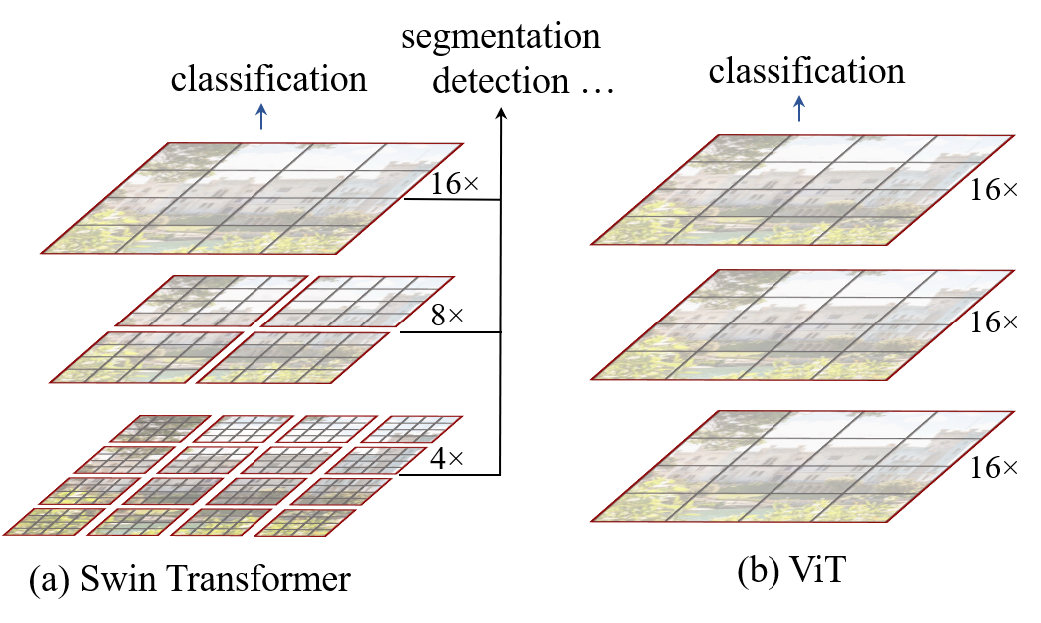
\includegraphics[width=0.75\linewidth]{gambar/swin-vs-vit.png}
	\caption{Perbedaan Arsitektur Swin Transformer dengan ViT \parencite{Liu2021}}
	\label{fig:vit-vs-swin}
\end{figure}

Berbeda dengan ViT yang menghasilkan pemetaan fitur dengan resolusi tunggal dan memiliki kompleksitas kuadratik seperti yang ditunjukkan pada Gambar \ref{fig:vit-vs-swin}, Swin Transformer membangun representasi hierarkis dengan kompleksitas linear terhadap ukuran gambar \textit{input}. Karakteristik hierarkis ini dicapai dengan memulai \textit{patch} dengan ukuran kecil yang secara bertahap digabungkan dengan \textit{patch} tetangga pada jaringan yang lebih dalam (\textit{patch merging}). Hal ini memungkinkan model untuk menggunakan teknik-teknik \textit{dense prediction} seperti \textit{Feature Pyramid Network} (FPN) atau U-Net \parencite{Liu2021}.

\begin{figure}[H]
	\centering
	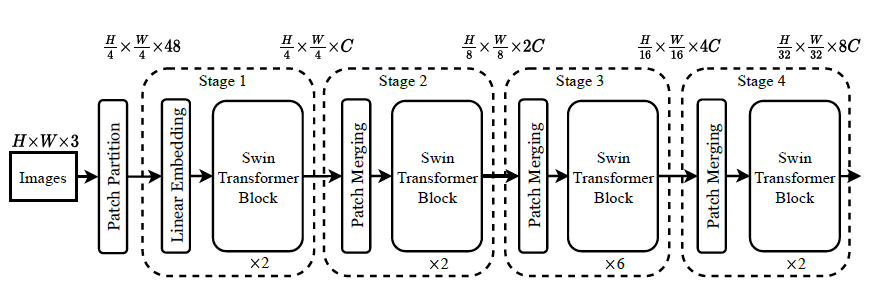
\includegraphics[width=\linewidth]{gambar/swin.png}
	\caption{Arsitektur Swin Transformer \parencite{Liu2021}}
	\label{fig:swin-arch}
\end{figure}

Berdasarkan arsitektur Swin pada Gambar \ref{fig:swin-arch}, proses dimulai dengan membagi gambar RGB \textit{input} menjadi \textit{patch} yang tidak tumpang tindih berukuran $4\times4$ piksel melalui modul \textit{patch partition} dengan fitur yang merupakan penggabungan (\textit{concantenation}) dari nilai RGB mentah setiap piksel. Setiap \textit{patch} diperlakukan sebagai token dan diproyeksikan secara linear ke dimensi tertentu ($C$). Arsitektur ini terdiri dari empat tahapan dengan setiap tahap kecuali tahap pertama diawali dengan \textit{patch merging layer} yang menggabungkan $2\times2$ \textit{patch} tetangga untuk mengurangi jumlah token sebanyak 4 kali dan meningkatkan dimensi fitur sebanyak 2 kali \parencite{Liu2021}.

Mekanisme \textit{Shifted Window based Self-Attention} menjadi keunggulan utama dari Swin Transformer dibandingkan dengan ViT. \textit{Attention} dihitung secara lokal di dalam \textit{windows} berukuran $M \times M$ yang membagi gambar secara merata tanpa tumpang tindih untuk efisiensi. Untuk menambahkan koneksi antar \textit{window} tanpa menambah beban komputasi, digunakan skema \textit{shifted windowing} pada blok Transformer yang berurutan. Blok pertama menggunakan partisi \textit{window} reguler, sedangkan blok berikutnya menggunakan konfigurasi partisi \textit{shifted window} sehingga informasi dapat melewati batas-batas \textit{window} pada \textit{layer} sebelumnya \parencite{Liu2021}.

Swin Transformer V2 dikembangkan untuk meningkatkan kapasitas model dan resolusi \textit{window} pada model sebelumnya \parencite{Liu2022}. \autoref{fig:swinv2} menunjukkan perbedaan arsitektur dengan versi sebelumnya. Versi ini mengatasi masalah ketidakstabilan pelatihan pada model besar dan perbedaan resolusi antara fase \textit{pre-training} dan \textit{fine-tuning} melalui tiga teknik utama:

\begin{enumerate}[nolistsep]
	\item \textit{Residual post-normalization}, mengganti konfigurasi \textit{pre-norm} dengan memindahkan lapisan \textit{Layer Normalization} (LN) ke bagian akhir setiap unit residual untuk mencegah ledakan nilai aktivasi pada lapisan yang lebih dalam.

	\item \textit{Scaled cosine attention}, mengganti \textit{dot product attention} dengan fungsi \textit{scaled cosine attention} agar nilai \textit{attention} tidak didominasi oleh amplitudo input tertentu yang menyebabkan ketidakstabilan pelatihan.

	\item \textit{Log-spaced continuous position bias}, mengganti optimasi \textit{parameterized bias} dengan jaringan meta kecil yang menggunakan koordinat \textit{log-spaced} dibandingkan dengan koordinat linear pada model terdahulu. Teknik ini memungkinkan model untuk melakukan transfer nilai \textit{bias} secara efektif meskipun ukuran resolusi \textit{window} berbeda jauh dengan pelatihan awal.
\end{enumerate}

\begin{figure}[H]
	\centering
	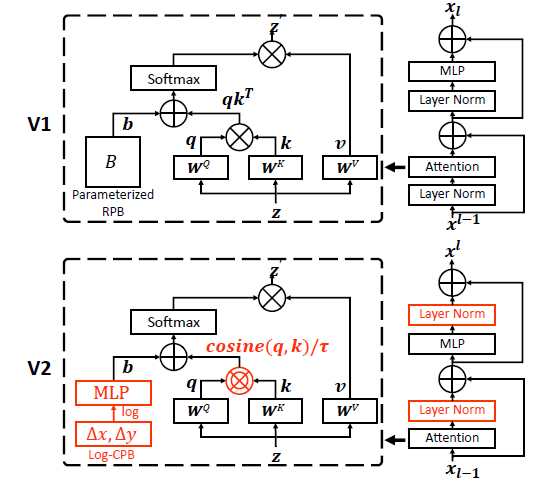
\includegraphics[width=0.47\linewidth]{gambar/swinv2.png}
	\caption{Perbedaan Swin Transformer V2 dengan V1 \parencite{Liu2022}}
	\label{fig:swinv2}
\end{figure}

Penggunaan teknik-teknik tersebut membuat Swin Transformer V2 menjadi model \textit{dense vision} terbesar yang mampu menangani resolusi gambar hingga $1.536 \times 1.536$ piksel dengan kinerja yang melampaui standar arsitektur sebelumnya.

%\subsection{DeiT}

\subsection{Pyramid Vision Transformer (PVT)}

Pyramid Vision Transformer (PVT) diperkenalkan sebagai model \textit{backbone} Transformer serbaguna yang dapat digunakan untuk tugas-tugas pada \textit{computer vision} tanpa bergantung pada operasi konvolusi \parencite{Wang2021}. PVT mengadopsi struktur piramida yang memungkinkan pembentukan \textit{multi-scale feature maps} yang serupa dengan struktur hierarkis pada CNN, seperti yang ditunjukkan pada \autoref{fig:pvt}.

\begin{figure}[H]
	\centering
	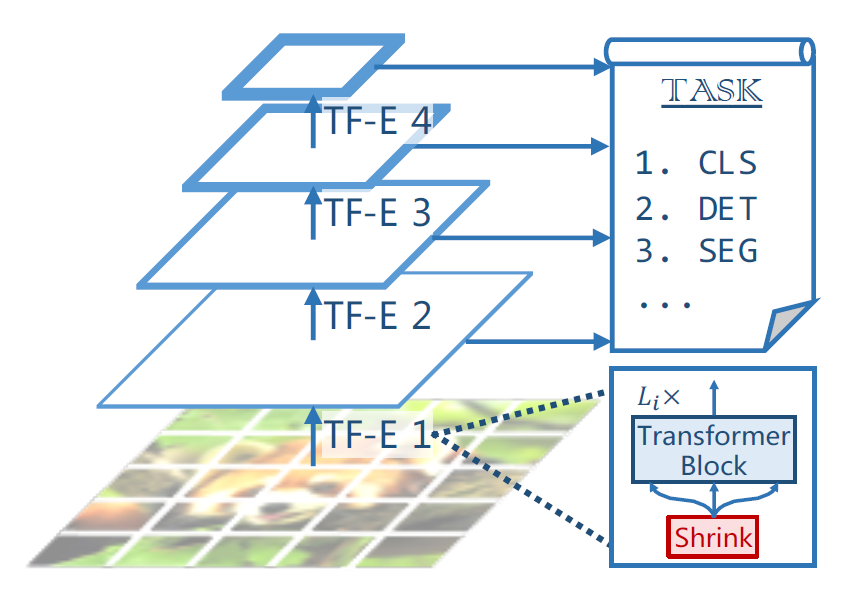
\includegraphics[width=0.6\linewidth]{gambar/pvt.png}
	\caption{Arsitektur Piramida pada PVT \parencite{Wang2021}}
	\label{fig:pvt}
\end{figure}

Model ini memperkenalkan strategi \textit{progressive shrinking} untuk mengontrol \textit{scaled feature map} melalui lapisan \textit{patch embedding}. PVT menggunakan mekanisme \textit{Spatial-Reduction Attention} (SRA) yang menggantikan \textit{Multi-Head Attention} (MHA) standar. SRA bekerja dengan cara mengurangi dimensi spasial dari matriks \textit{Key} (K) dan \textit{Value} (V) sebelum operasi \textit{attention} dilakukan sehingga dapat mengurangi konsumsi sumber daya komputasi dan memori secara signifikan.

PVT v2 diperkenalkan sebagai pengembangan untuk mengatasi keterbatasan pada versi sebelumnya seperti kompleksitas komputasi yang masih tinggi pada resolusi besar dan hilangnya kontinuitas lokal. Berikut adalah tiga perbedaan utama pada PVT v2 yang menyempurnakan arsitektur sebelumnya.

\begin{enumerate}[nolistsep]
	\begin{figure}[H]
		\centering
		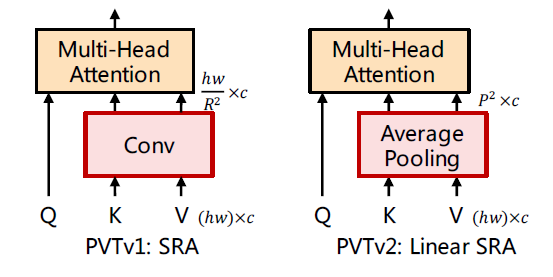
\includegraphics[width=0.5\linewidth]{gambar/pvt-vs-v2.png}
		\caption{Perbandingan Mekanisme SRA pada PVT v1 dan \textit{Linear} SRA pada PVT v2  \parencite{Wang2023}}
		\label{fig:lsra-pvt2}
	\end{figure}

	\item \textit{Linear Spatial-Reduction Attention} (LSRA), ditunjukkan pada Gambar \ref{fig:lsra-pvt2} yang menggantikan \textit{layer} konvolusi dengan menggunakan \textit{average pooling} untuk mengurangi dimensi spasial menjadi ukuran tetap ($P \times P$) Hal ini memungkinkan komputasi dan memori yang linear terhadap ukuran \textit{input} gambar yang serupa dengan efisiensi pada \textit{layer} konvolusi.

	\begin{figure}[H]
		\centering
		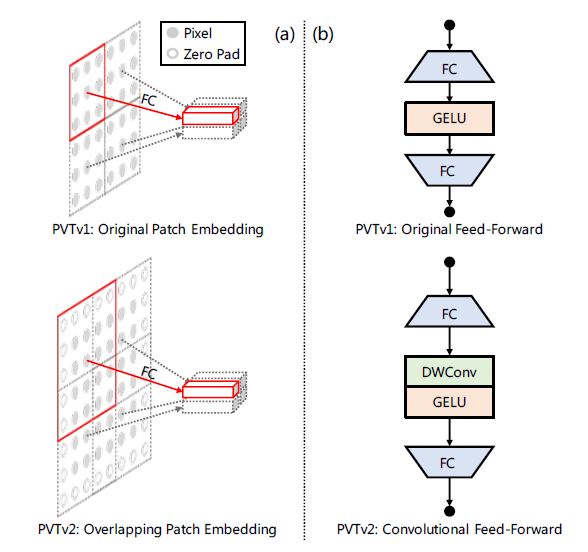
\includegraphics[width=0.57\linewidth]{gambar/pvt-v2-improv.png}
		\caption{Mekanisme \textit{Overlapping Patch Embedding} dan \textit{Convolutional Feed-Forward Network}  \parencite{Wang2023}}
		\label{fig:pvt-v2}
	\end{figure}

	\item \textit{Overlapping Patch Embedding} (OPE), PVT v2 menggunakan konvolusi dengan \textit{zero padding} untuk mengimplementasikan \textit{patch embedding} yang saling tumpang tindih, seperti yang ditunjukkan pada \autoref{fig:pvt-v2}. Dengan memperbesar \textit{patch window} sehingga setengah area \textit{window} yang berdekatan saling tumpang tindih, model mampu menangkap informasi kontinuitas lokal dari gambar dan \textit{feature map} lebih baik dibandingkan metode \textit{non-overlapping} pada PVT v1.

	\item \textit{Convolutional Feed-Forward Network} (CFFN), PVT v2 menambahkan \textit{depth-wise convolution layer} berukuran $3 \times 3$ dengan \textit{zero padding} di dalam \textit{feed-forward network} untuk meningkatkan kemampuan ekstraksi fitur lokal, seperti yang ditunjukkan pada \autoref{fig:pvt-v2}. Penambahan ini tidak hanya menangkap kontinuitas lokal pada \textit{input tensor}, tetapi juga memberikan informasi posisi secara implisit sehingga penggunaan \textit{fixed-size positional encoding} yang tidak fleksibel pada versi sebelumnya dapat dihilangkan.

\end{enumerate}

Perubahan ketiga komponen ini membuat PVT v2 mampu memproses input dengan resolusi variabel secara lebih fleksibel sekaligus mencapai kinerja yang lebih unggul dibandingkan \textit{backbone} CNN maupun Transformer lainnya pada berbagai tugas \textit{computer vision}.

\subsection{\textit{Large Language Model}}

\textit{Large Language Model} (LLM) merupakan model bahasa berbasis arsitektur Transformer yang memiliki jumlah parameter yang sangat banyak, umumnya berjumlah hingga miliaran dan dilatih menggunakan korpus data tekstual yang besar. Karakteristik utama yang membedakan LLM dari model bahasa konvensional adalah munculnya \textit{emergent abilities}, yaitu kemampuan cerdas seperti penalaran kompleks, pemecahan masalah matematika, dan pembelajaran dalam konteks (\textit{in-context learning}) yang muncul secara spontan setelah model mencapai skala data dan parameter tertentu \parencite{Zhao2025}.

LLM umumnya dibangun menggunakan arsitektur Transformer \textit{decoder} yang menggunakan mekanisme \textit{self-attention} untuk memodelkan hubungan antar elemen dalam urutan data secara paralel \parencite{Cheng2025}. Prinsip utama LLM adalah melakukan pemodelan bahasa melalui prediksi token berikutnya (\textit{next-token prediction}). Dalam proses ini, model menghitung probabilitas generatif dari urutan kata untuk memprediksi token berikutnya berdasarkan konteks sebelumnya \parencite{Zhao2025}. LLM menggunakan tumpukan \textit{multi-head attention layer} dan \textit{feed-forward network} untuk belajar memadatkan pengetahuan ke dalam parameter-parameter jaringan dengan tujuan sebagai pemecah masalah generik (\textit{general-purpose task solver}) \parencite{Cheng2025, Zhao2025}. Seiring perkembangan teknologi, muncul varian baru LLM yaitu \textit{Multimodal Large Language Model} (MLLM) yang mampu mengintegrasikan dan memproses berbagai modalitas informasi seperti teks, citra, dan video. Struktur umum MLLM terdiri dari tiga komponen inti, yaitu \textit{Vision Encoder} untuk melakukan ekstraksi fitur visual, \textit{Cross-modal Connector} untuk menyelaraskan fitur visual ke dalam ruang semantik teks, dan LLM \textit{Backbone} sebagai unit penalaran utama \parencite{Wang2024}.

Untuk menyesuaikan kapabilitas umum model dengan kebutuhan spesifik, LLM menggunakan dua mekanisme adaptasi:

\begin{enumerate}[nolistsep]
	\item \textit{Instruction tuning}, merupakan pendekatan \textit{fine-tuning pre-trained} LLM menggunakan kumpulan data yang diformat dalam bentuk bahasa alami (\textit{natural language}) \parencite{Zhao2025}. Proses ini bertujuan untuk memperbarui bobot internal model agar dapat beradaptasi untuk mengikuti perintah spesifik dan memahami logika pada deskripsi tugas sehingga meningkatkan kemampuan generalisasi pada tugas-tugas yang belum pernah ditemui sebelumnya \parencite{Cheng2025, Zhao2025, Brickman2025}.

	\item \textit{Prompt engineering}, strategi ini dilakukan pada saat inferensi tanpa mengubah parameter internal model \parencite{Zhao2025}. Teknik ini berfokus pada perancangan instruksi input yang optimal seperti \textit{zero-shot prompting} tanpa menggunakan contoh atau \textit{few-shot prompting} dengan memberikan beberapa contoh pasangan \textit{input-output}. Hal ini bertujuan untuk mengeksplorasi pengetahuan yang sudah tersimpan di dalam model secara maksimal \parencite{Brickman2025}.
\end{enumerate}

\subsection{\textit{Prompt Engineering}}

\textit{Prompt engineering} didefinisikan sebagai sekumpulan teknik dan metode untuk merancang, menulis, dan mengoptimalkan instruksi guna memastikan respons LLM bersifat akurat, relevan, dan bebas dari informasi yang menyesatkan. Strategi ini bekerja pada fase inferensi dengan memanfaatkan pengetahuan yang telah tersimpan di dalam parameter model tanpa melakukan \textit{update} bobot internal \parencite{Brickman2025}. Desain \textit{prompt} yang mencakup kejelasan instruksi, penyediaan konteks, serta kontrol terhadap format \textit{output} yang diinginkan dapat meningkatkan akurasi interaksi LLM sesuai dengan konteks yang diharapkan \parencite{Velsquez-Henao2023}.

Salah satu teknik yang \textit{prompting} yang umum digunakan adalah \textit{role-play prompting}, yaitu ketika model diminta untuk memerankan suatu persona tertentu, seperti menjadi seorang guru matematika atau hakim yang adil \parencite{Kong2024}. Pemberian peran ini berfungsi untuk membatasi ruang lingkup identitas model dan membantu memberikan pengetahuan parametrik yang relevan sehingga respons yang dihasilkan lebih natural dan selaras dengan tugas spesifik \parencite{Tseng2024, Kong2024}. Selain meningkatkan keterlibatan pengguna, penelitian menunjukkan bahwa \textit{role-play prompting} dapat berfungsi sebagai pemicu implisit bagi mekanisme \textit{Chain-of-Thought} (CoT) yang memperkuat kemampuan penalaran model dibandingkan dengan instruksi standar \parencite{Kong2024}.

Teknik lain yang digunakan adalah \textit{contextual injection}, yaitu proses mengintegrasikan data atau informasi latar belakang yang spesifik ke dalam prompt untuk memandu model dalam menghasilkan jawaban \parencite{Velsquez-Henao2023, Zhao2025}. Penggunaan informasi kontekstual sangat penting dalam domain khusus seperti teknik atau medis ketika model membutuhkan data presisi guna menghindari fenomena halusinasi atau jawaban yang terlalu umum. Injeksi konteks dapat diimplementasikan dengan melampirkan dokumen referensi, struktur data organisasi, maupun instruksi mendetail mengenai batasan tugas yang harus diselesaikan oleh sistem \parencite{Velsquez-Henao2023}. Melalui kombinasi identitas peran dan penyediaan data kontekstual yang sesuai, LLM mampu berfungsi sebagai asisten cerdas yang memberikan solusi yang valid secara faktual dan tepat \parencite{Tseng2024}.

\subsection{Gemma}

Gemma merupakan salah satu model \textit{open source} yang dikembangkan oleh Google DeepMind menggunakan penelitian dan teknologi yang sama dengan model Gemini. Model ini dirancang dalam berbagai ukuran untuk memfasilitasi keterbatasan sumber daya komputasi sehingga dapat dijalankan pada perangkat keras kelas konsumen seperti laptop yang hanya menggunakan CPU. Gemma dibangun di atas arsitektur Transformer \textit{decoder} yang mendukung panjang konteks dari 8192 token hingga 256.000 token pada model terbaru. Arsitektur Gemma mengintegrasikan berbagai pendekatan modern untuk menjaga efisiensi dan stabilitas pelatihan seperti penggunaan \textit{Rotary Positional Embeddings} (RoPE), aktivasi GeGLU, serta normalisasi RMSNorm \parencite{GemmaTeam2024}. Model terbaru, yaitu Gemma 4 tersedia dalam 3 varian, yaitu \textit{Small} (2B dan 4B), \textit{Dense} (31B), dan \textit{Mixture-of-Experts} (26B A4B) yang memungkinkan fleksibilitas penggunaan sesuai dengan batasan daya komputasi perangkat yang digunakan \parencite{Gemma4Model}.

Gemma menunjukkan kinerja yang unggul pada NLP, penalaran umum, serta tugas-tugas analitis yang kompleks. Model ini mencapai kinerja \textit{state-of-the-art} pada berbagai bidang seperti matematika, sains, dan pemrograman. Varian Gemma 3 memperkenalkan kemampuan multimodal yang memungkinkan model untuk memahami input visual secara langsung melalui integrasi SigLIP \textit{vision encoder}. Kemampuan visual tersebut didukung oleh metode \textit{Pan and Scan} (P\&S) yang membuat model mampu menangkap gambar pada resolusi dan rasio aspek aslinya tanpa kehilangan detail penting atau teks yang berukuran kecil. Selain itu, untuk mengoptimalkan penggunaan memori saat menangani konteks data yang sangat panjang, Gemma menerapkan mekanisme \textit{interleaving} dengan rasio 5:1 antara lapisan \textit{self-attention} lokal dan global. Seluruh varian model Gemma juga melalui proses \textit{instruction-tuning} dan \textit{Reinforcement Learning from Human Feedback} (RLHF) untuk memastikan tingkat keselarasan respon yang tinggi terhadap preferensi pengguna manusia \parencite{GemmaTeam2025}.

\subsection{Qwen-VL}

Qwen-VL merupakan \textit{Large Vision-Language Model} (LVLM) yang dikembangkan oleh tim Alibaba Cloud untuk memahami informasi tekstual serta visual secara simultan. Arsitektur dasar model ini terdiri dari tiga komponen utama, yaitu LLM Qwen sebagai unit penalaran, \textit{vision encoder} berbasis ViT-bigG, serta \textit{Vision-Language Adapter} yang menggunakan mekanisme \textit{cross-attention} untuk memproses fitur visual secara efisien. Model ini menggunakan pengkodean posisi absolut 2D untuk memitigasi hilangnya detail spasial selama proses kompresi fitur serta jalur pelatihan tiga tahap yang meliputi penyelarasan visi-bahasa, pelatihan multi-tugas pada korpus multibahasa, dan penyetelan instruksi visual. Kapabilitas utama Qwen-VL mencakup deskripsi citra (\textit{image captioning}), \textit{Visual Question Answering}(VQA), \textit{Optical Character Recognition} (OCR) tingkat lanjut, serta \textit{visual grounding} \parencite{Bai2023}.

Model versi terbaru yaitu Qwen3-VL mempunyai kemampuan pemahaman konteks multimodal yang dapat memproses hingga 256.000 token yang mencakup teks, gambar, dan video. Model ini dikenalkan dalam beberapa varian, mulai dari arsitektur \textit{dense} dengan 2B hingga 32B parameter, hingga arsitektur \textit{Mixture-of-Experts}, serta menyediakan varian \textit{thinking} yang difokuskan pada kemampuan penalaran multimodal yang kompleks. Qwen3-VL membawa tiga pembaruan arsitektur utama, yaitu penerapan \textit{interleaved-MRoPE} yang mendistribusikan komponen spasial dan temporal secara seragam untuk memperbaiki bias spektrum frekuensi sehingga pemodelan video menjadi lebih representatif, integrasi mekanisme \textit{DeepStack} yang mengekstrak dan menggabungkan fitur visual dari berbagai lapisan Vision Transformer secara langsung pada \textit{layer} LLM untuk memperkuat penyelarasan visi-bahasa dengan mempertahankan kekayaan detail dari level rendah hingga tinggi, serta transisi dari metode T-RoPE ke penyelarasan \textit{textual timestamp} secara eksplisit untuk penyelarasan waktu berbasis teks untuk video, yang memberikan pemahaman struktur waktu (\textit{temporal grounding}) yang lebih presisi \parencite{Bai2025Qwen3}.

% TODO: Tinjauan Pustaka
%\subsection{Antarmuka Pengguna}

%\subsection{\textit{Application Programming Interface} (API)}

\subsection{Metrik Evaluasi}

Pada bagian ini, akan dijelaskan metrik evaluasi yang digunakan untuk mengukur kinerja model dalam menghasilkan prediksi dan interpretasi. Evaluasi dilakukan untuk menilai seberapa akurat hasil prediksi model regresi dan interpretasi LLM dalam menilai kepribadian.

\subsubsection{Metrik Evaluasi Model Prediksi}

Kualitas model pada tugas regresi untuk memprediksi skor kepribadian \textit{Big Five} tidak dievaluasi dengan akurasi klasifikasi, tetapi dengan seberapa dekat nilai prediksi terhadap skor kontinu \textit{ground truth}. Oleh karena itu, digunakan kombinasi metrik \textit{error} (MAE, RMSE), metrik varians (R²), dan \textit{Accuracy} (1–MAE) yang memetakan \textit{error} menjadi nilai kemiripan yang mudah ditafsirkan \parencite{Plevris2022, Chicco2021}.

\begin{enumerate}[nosep, label=\alph*.]
	\item \textit{Mean Absolute Error} (MAE) \\
	MAE mengukur rata-rata \textit{error} absolut antara nilai sebenarnya dan nilai prediksi yang ditunjukkan pada Persamaan \ref{eq:mae}.
	\begin{equation}
		\text{MAE} = \frac{1}{N}\sum_{i=1}^{N} | y_i - \hat{y}_i |
		\label{eq:mae}
	\end{equation}
	dengan $y_i$ merupakan skor kepribadian aktual, $\hat{y}_i$ adalah skor prediksi, dan $N$ jumlah sampel. MAE tidak membedakan arah kesalahan (\textit{over/under‑estimate}) dan kurang sensitif terhadap \textit{outlier} dibanding metrik berbasis kuadrat sehingga sering digunakan sebagai indikator umum \textit{error} rata‑rata model regresi \parencite{Chicco2021}. MAE yang lebih kecil berarti prediksi skor rata-rata tiap \textit{Big Five trait} lebih dekat ke nilai sebenarnya.
	\item \textit{Accuracy} \\
	Kompetisi ChaLearn menggunakan metrik \textit{Accuracy} untuk mendapatkan nilai antara 0-1 yang interpretasinya mirip dengan metrik akurasi pada klasifikasi tetapi tetap berbasis \textit{error} kontinu. Rumus \textit{Accuracy} ditunjukkan pada Persamaan \ref{eq:accuracy}.
	\begin{equation}
		\text{Accuracy} = 1 - \text{MAE}_\text{model}
		\label{eq:accuracy}
	\end{equation}
	di mana $\text{MAE}_\text{model}$ adalah MAE dari hasil prediksi model. Metrik ini digunakan sebagai metrik utama yang hasilnya dapat diintepretasikan dengan lebih mudah \parencite{Ponce-Lpez2016}.
	\item \textit{Root Mean Square Error} (RMSE) \\
	RMSE mengukur rata‑rata \textit{error} dengan memberi bobot lebih besar pada error yang besar seperti ditunjukkan pada Persamaan \ref{eq:rmse}.
	\begin{equation}
		\text{RMSE} = \sqrt{\frac{1}{N}\sum_{i=1}^{N} (y_i - \hat{y}_i)^2}
		\label{eq:rmse}
	\end{equation}
	RMSE selalu lebih besar dari MAE dan sangat berguna ketika \textit{error} besar dianggap lebih penting karena \textit{error} dikuadratkan sebelum dirata-rata \parencite{Chai2014}. Dalam prediksi kepribadian \textit{Big Five}, RMSE yang rendah menunjukkan bahwa model tidak hanya baik secara rata‑rata, tetapi juga jarang menghasilkan prediksi yang sangat jauh dari nilai aktual.
	\item \textit{Coefficient of Determination} ($R^{2}$)  \\
	\textit{Coefficient of determination} atau $R^{2}$ mengukur proporsi varians target yang dapat dijelaskan model dibandingkan \textit{baseline} yang hanya memprediksi rata‑rata, dihitung dengan Persamaan \ref{eq:rsquare}.
	\begin{equation}
		R^{2} = 1 - \frac{\sum_{i=1}^{N} (y_i - \hat{y}i)^2}{\sum_{i=1}^{N} (y_i - \bar{y})^2}
		\label{eq:rsquare}
	\end{equation}
	dengan $\bar{y}$ adalah rata‑rata skor kepribadian aktual. Nilai $R^{2}$ bisa negatif yang berarti model lebih buruk dari \textit{baseline} rata‑rata hingga 1 yang berarti \textit{fit} sempurna. $R^{2}$ yang lebih tinggi berarti model menjelaskan porsi lebih besar variasi skor kepribadian antar individu. Dalam prediksi kepribadian \textit{Big Five}, $R^{2}$ sering dipakai berdampingan dengan RMSE. RMSE menyatakan besarnya \textit{error} dalam satuan skor, sedangkan $R^{2}$ menyatakan seberapa baik model menjelaskan struktur varians data \parencite{Chicco2021, Habib2024}.
\end{enumerate}

\subsubsection{G-Eval}

G-Eval merupakan kerangka kerja evaluasi berbasis LLM yang dirancang untuk menilai kualitas teks hasil generasi menggunakan mekanisme \textit{Chain-of-Thought} (CoT) dan paradigma \textit{form-filling} \parencite{Liu2023}. Pada ekosistem pengembangan kecerdasan buatan, G-Eval menjadi representasi dari paradigma \textit{LLM-as-a-judge} yang memanfaatkan LLM seperti GPT-4 sebagai otoritas penilai untuk memberikan skor, peringkat, atau seleksi terhadap \textit{output} model lain \parencite{Li2025}. Keunggulan utama G-Eval dibandingkan metrik tradisional seperti BLEU atau ROUGE adalah kemampuannya untuk menangkap atribut semantik yang kompleks dan nuansa konteks yang sering kali lolos dari pengukuran berbasis \textit{lexical overlap} \parencite{Pereira2024}.

Kerangka kerja G-Eval diimplementasikan secara sistematis melalui integrasi tiga komponen utama yang ditunjukkan pada Gambar \ref{fig:g-eval}. Proses ini diawali dengan penyusunan \textit{prompt} yang berisi pengenalan tugas serta definisi kriteria evaluasi spesifik untuk memberikan batasan parameter bagi LLM yang bertindak sebagai otoritas penilai \parencite{Liu2023}. Selanjutnya, model menjalankan mekanisme \textit{Auto Chain-of-Thought} (Auto-CoT) untuk menghasilkan rangkaian langkah evaluasi internal secara otomatis yang berfungsi memberikan panduan penalaran secara detail bagi model sebelum memberikan skor akhir \parencite{Chiang2023}. Berdasarkan panduan langkah tersebut, model kemudian memproses teks target melalui paradigma \textit{form-filling} untuk menghasilkan prediksi kualitas \textit{output}. G-Eval tidak hanya mengambil skor integer mentah, melainkan menggunakan fungsi penilaian berbobot yang memanfaatkan probabilitas dari token \textit{output} model untuk melakukan normalisasi sehingga menghasilkan skor kontinu yang mampu menangkap nuansa perbedaan kualitas dengan lebih halus \parencite{Liu2023}. Pada tahap akhir untuk menjamin reliabilitas hasil, kerangka kerja ini menerapkan strategi \textit{self-consistency }dengan melakukan pengambilan sampel berulang dan menghitung rata-rata skor untuk memitigasi bias distribusi dan memastikan keselarasan yang tinggi dengan penilaian manusia \parencite{Pereira2024}.

\begin{figure}[H]
	\centering
	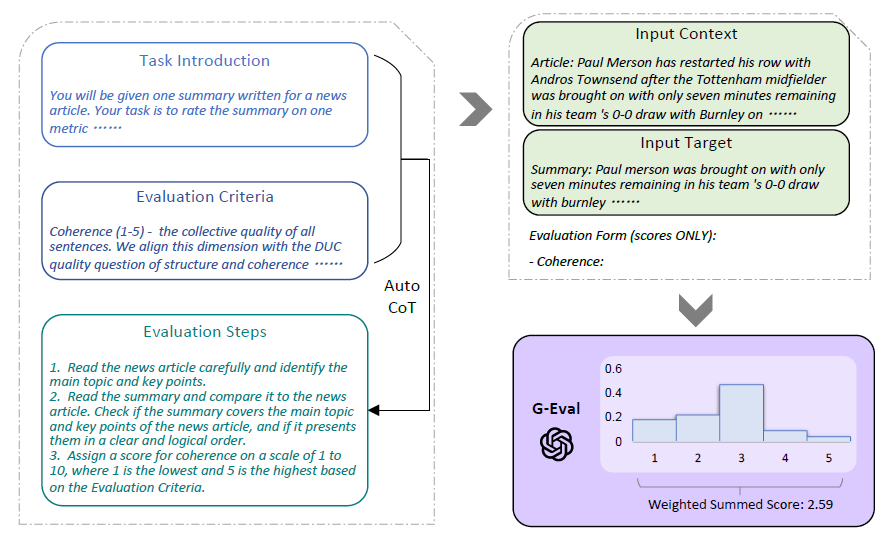
\includegraphics[width=0.9\linewidth]{gambar/g-eval.png}
	\caption{Kerangka Kerja G-Eval \parencite{Liu2023}}
	\label{fig:g-eval}
\end{figure}